%%%%%%%%%%%%%%%%%%%%%%%%%%%%%%%%%%%%%%%%%%%%%%%%%%%%%%%%%%%%%%%%%%%%%%
% (latex Lep2wgInt; dvips Lep2wgInt.dvi)
% ghostview -bg white -fg black  -magstep -1 Lep2wgInt.ps&
%%%%%%%%%%%%%%%%%%%%%%%%%%%%%%%%%%%%%%%%%%%%%%%%%%%%%%%%%%%%%%%%%%%%%%
%%%%%%%%%%%%%%%%%%%%%%%%%%%%%%%%%%%%%%%%%%%%%%%%%%%%%%%%%%%%%%%%%%%%%%
\documentclass[dvips,portrait]{cernsem}             %%%%%%%%%%%%%%%%%%
                                                    %%%%%%%%%%%%%%%%%%


% AmsTeX package
\usepackage{amsmath}
\usepackage{amssymb}
\usepackage{euscript}
\usepackage{feynmf}
\usepackage{fancybox}

% The epsfig.sty is necessary to manage figures in postscript!
\usepackage{epsfig}



%%%%%%%%%%%%%%%%%%%%%%%%%%%%%%%%%%%%%%%%%%%%%%%%%%%%%%%
%
\def\halp{\hat{\alpha}}
\def\hbet{\hat{\beta}}
\def\Order#1{${\cal O}(#1$)}
\def\Ordpr#1{${\cal O}(#1)_{prag}$}
\def\Oeex#1{${\cal O}(#1)_{_{\rm EEX}}$}
\def\Oceex#1{${\cal O}(#1)_{_{\rm CEEX}}$}
\def\bbeta{\bar{\beta}}
\def\born{{\rm Born}}
\newcommand{\KK}{${\cal KK}$}
\def\Energy{189GeV}
\def\Angle{$\theta^{\bullet}$}
%

%\pagecolor{Yellow}
\pagecolor{Goldenrod}
\SlideColours{black}{white}
\renewcommand{\slidestretch}{0.8}

\title{ CERN LEP2 WG}
\author{Stanis\l{}aw Jadach, B.F.L. Ward and Z. Was}
\date{\small 28 May, 1999}

\renewcommand{\Semlabel}{DESY}


%%%%%%%%%%%%%%%%%%%%%%%%%%%%%%%%%%%%%%%%%%%%%%%%%%%%%%%
%%%%%%%%%%%%%%%%%%%%%%%%%%%%%%%%%%%%%%%%%%%%%%%%%%%%%%%
\begin{document}                     %%%%%%%%%%%%%%%%%%



%%%%%%%%%%%%%%%%%%%%%%%%%%%%%%%%%%%%%%%%%%%%%%%%%%%%%%%%%%%%%%%%%%%%%%%%%%%%%
%%%%%%%%%%%%%%%%%%%%%%%%%%%%%%%%%%%%%%%%%%%%%%%%%%%%%%%%%%%%%%%%%%%%%%%%%%%%%
                                                         %%%%%%%%%%%%%%%%%%%%
\begin{Slide}{{\bf\color{red} ISR*FSR Interference from \KK\ MC generator }}

%%%%\begin{center}
%%%%{\bf\color{Black} S. Jadach, DESY and INP Cracow }
%%%%\end{center}
%%%%\begin{center}
%%%%{\bf\color{Black} In collaboration with Z. Was and B.F.L. Ward }
%%%%\end{center}

\begin{center}
{\bf\color{Black} S. JADACH, B.F.L. Ward and  Z. Was\\
CERN 28 May 1999, Meeting of LEP EWG}
\end{center}

\vspace{5mm}
QUESTIONS:
{\bf\color{blue}
  \begin{itemize}
  \item
    How big is ISR*FSR Interference in $\sigma_{tot}$ and $A_{FB}$?
  \item
    Do we know it at \Order{\alpha^1}?
  \item
    Do we know it beyond \Order{\alpha^1}?
  \item
    How sensitive it is to cut-off changes?
  \item
    Conclusions
  \end{itemize}
}

{\bf\color{Magenta}  For \KK\ MC check {\tt http://home.cern.ch/$\sim$jadach}}
\end{Slide}                               %%%%%%%%%%%%%%%%%%%%%%%%%%%%%%%%%%%
%%%%%%%%%%%%%%%%%%%%%%%%%%%%%%%%%%%%%%%%%%%%%%%%%%%%%%%%%%%%%%%%%%%%%%%%%%%%%










%%%%%%%%%%%%%%%%%%%%%%%%%%%%%%%%%%%%%%%%%%%%%%%%%%%%%%%%%%%%%%%%%%%%%%%%%%%%%
%%%%%%%%%%%%%%%%%%%%%%%%%%%%%%%%%%%%%%%%%%%%%%%%%%%%%%%%%%%%%%%%%%%%%%%%%%%%%
%%%%%%%%%%%%%%%%%%%%%%%%%%%%%%%%%%%%%%%%%%%%%%%%%%%%%%%%%%%%%%%%%%%%%%%%%%%%%
                                                         %%%%%%%%%%%%%%%%%%%%
\begin{PSlide}{{\small\color{Magenta} 
      ISR*FSR interf. in angular distribution}}

{\small\color{Blue}
  The influence of ISR*FSR  interference at \Energy. 
  The energy cut is on $s'/s$, where $s'=m^2_{f\bar{f}}$.
  The angular cut is $|\cos\theta|<\cos\theta_{\max}$}
{\small\color{Blue} Scattering angle is $\theta=$\Angle. }
{\tiny\color{Blue}  [Angle $\theta^{\bullet}$ is defined in Phys. Rev. {\bf D41}, 1425 (1990)]}

%-----------------------------------------------------------
\begin{center}
\setlength{\unitlength}{1mm}
%
\begin{picture}(35,35)
\put(-1, 0){\makebox(0,0)[lb]{
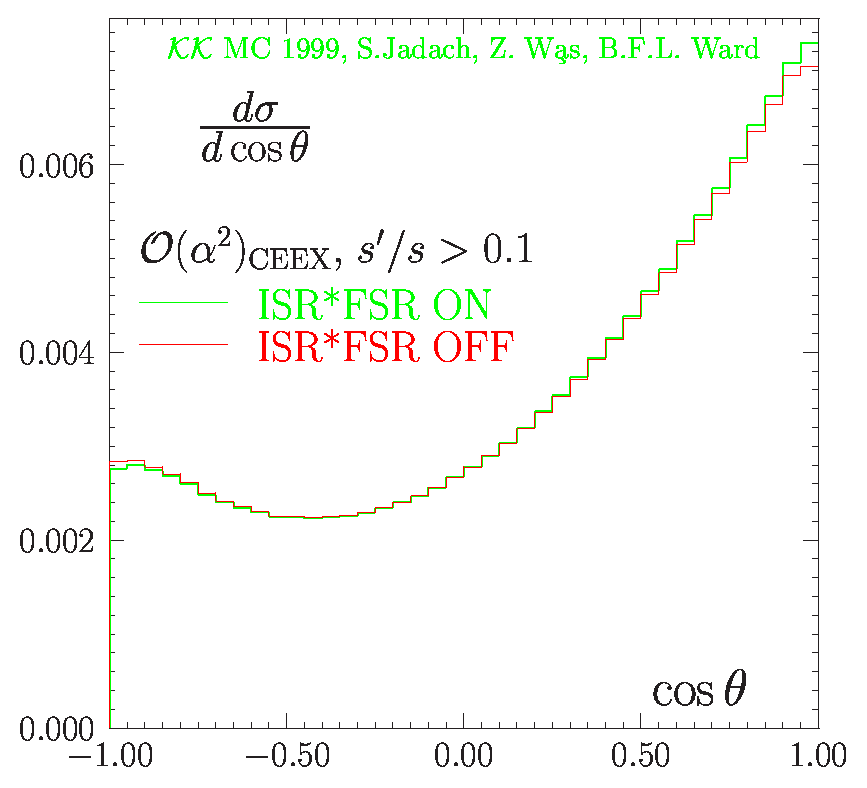
\epsfig{file=afb-int-G1.eps,width=35mm,height=34mm}
}}\end{picture}
%
\begin{picture}(35,35)
\put(-1, 0){\makebox(0,0)[lb]{
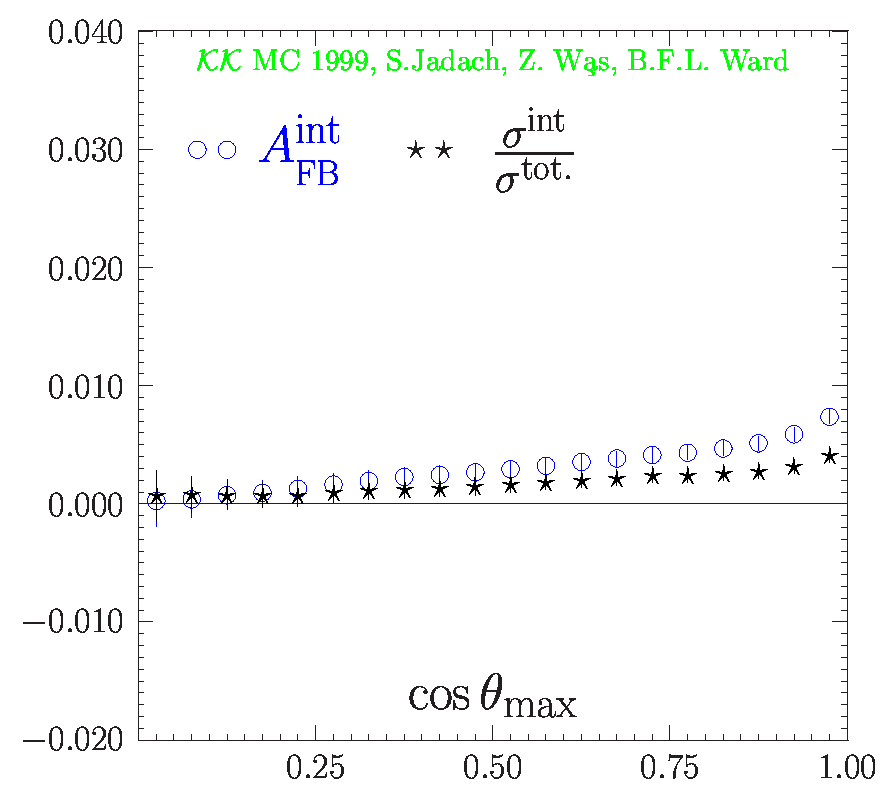
\epsfig{file=afb-int-com1.eps,width=35mm,height=34mm}
}}\end{picture}
%
\end{center}
%-----------------------------------------------------------
\begin{center}
\setlength{\unitlength}{1mm}
%
\begin{picture}(35,35)
\put(-1, 0){\makebox(0,0)[lb]{
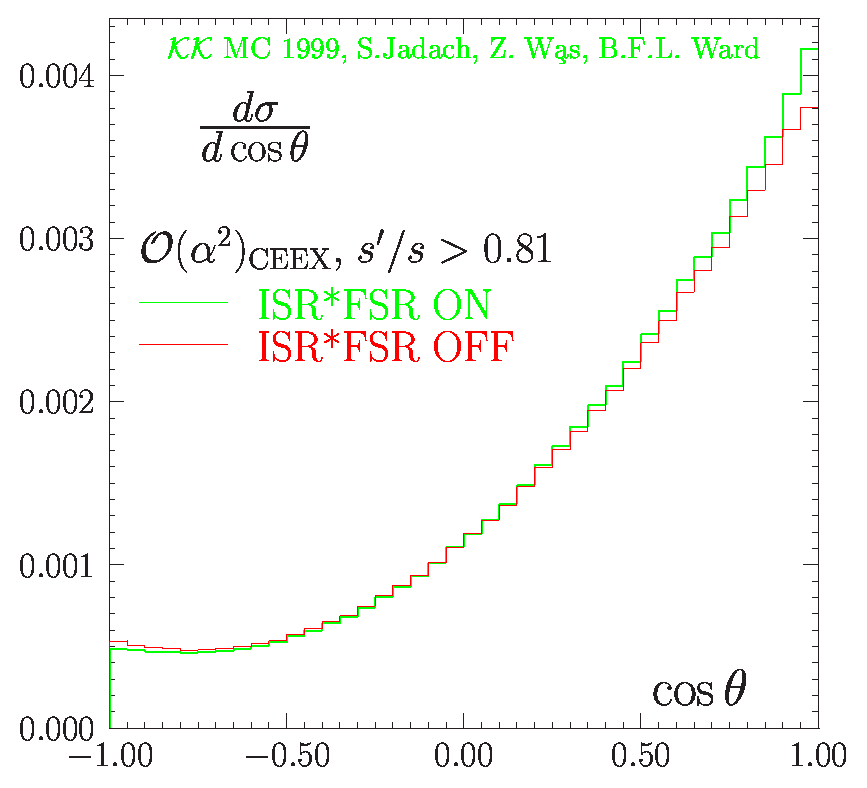
\epsfig{file=afb-int-G1x.eps,width=35mm,height=34mm}
}}\end{picture}
%
\begin{picture}(35,35)
\put(-1, 0){\makebox(0,0)[lb]{
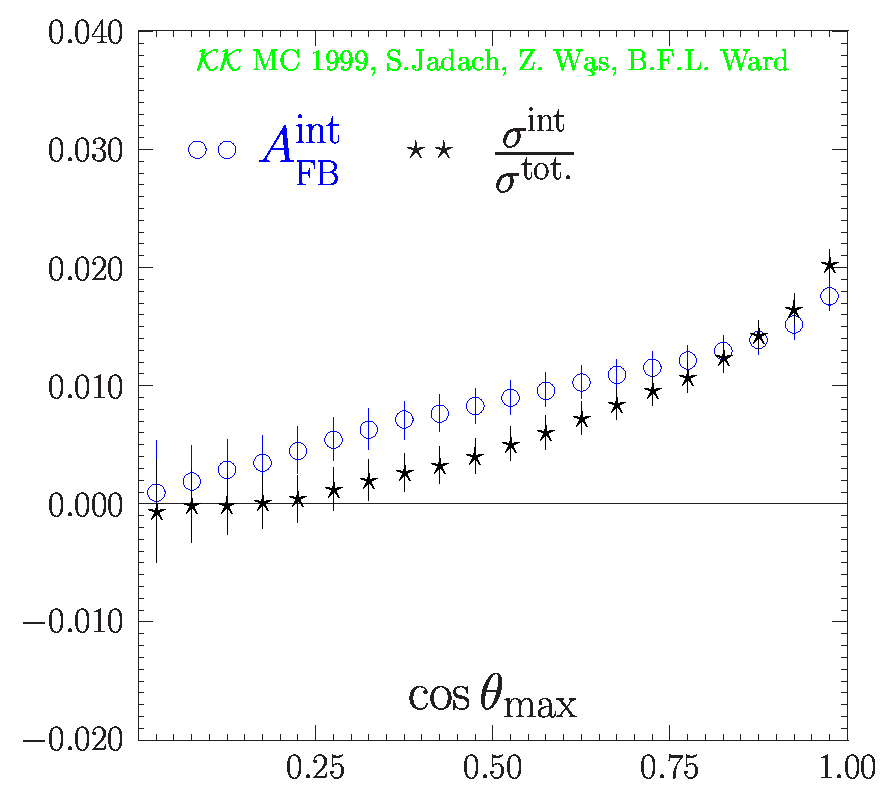
\epsfig{file=afb-int-com1x.eps,width=35mm,height=34mm}
}}\end{picture}
%
\end{center}
%-----------------------------------------------------------
\end{PSlide}
                                                         %%%%%%%%%%%%%%%%%%%%
%%%%%%%%%%%%%%%%%%%%%%%%%%%%%%%%%%%%%%%%%%%%%%%%%%%%%%%%%%%%%%%%%%%%%%%%%%%%%






%%%%%%%%%%%%%%%%%%%%%%%%%%%%%%%%%%%%%%%%%%%%%%%%%%%%%%%%%%%%%%%%%%%%%%%%%%%%%
%%%%%%%%%%%%%%%%%%%%%%%%%%%%%%%%%%%%%%%%%%%%%%%%%%%%%%%%%%%%%%%%%%%%%%%%%%%%%
%%%%%%%%%%%%%%%%%%%%%%%%%%%%%%%%%%%%%%%%%%%%%%%%%%%%%%%%%%%%%%%%%%%%%%%%%%%%%
                                                         %%%%%%%%%%%%%%%%%%%%
\begin{PSlide}{{\small\color{Magenta} 
      ISR*FSR in $\sigma$, cut-off dependence}}

{\small\color{ForestGreen}
  The ISR*FSR {\color{Red} interference} correction
  to $\sigma(s'_{\min})$ at \Energy.
  No cut in $\cos$\Angle.
  From {\color{red} \KK\ M.C. with \Oceex{\alpha^1} }
  exponentiation at the amplitude level.
}

\begin{center}
\setlength{\unitlength}{1mm}
\begin{picture}(65,60)
%#####\put(0,0){\framebox( 65,60){ }}
\put(-2, 00){\makebox(0,0)[lb]{
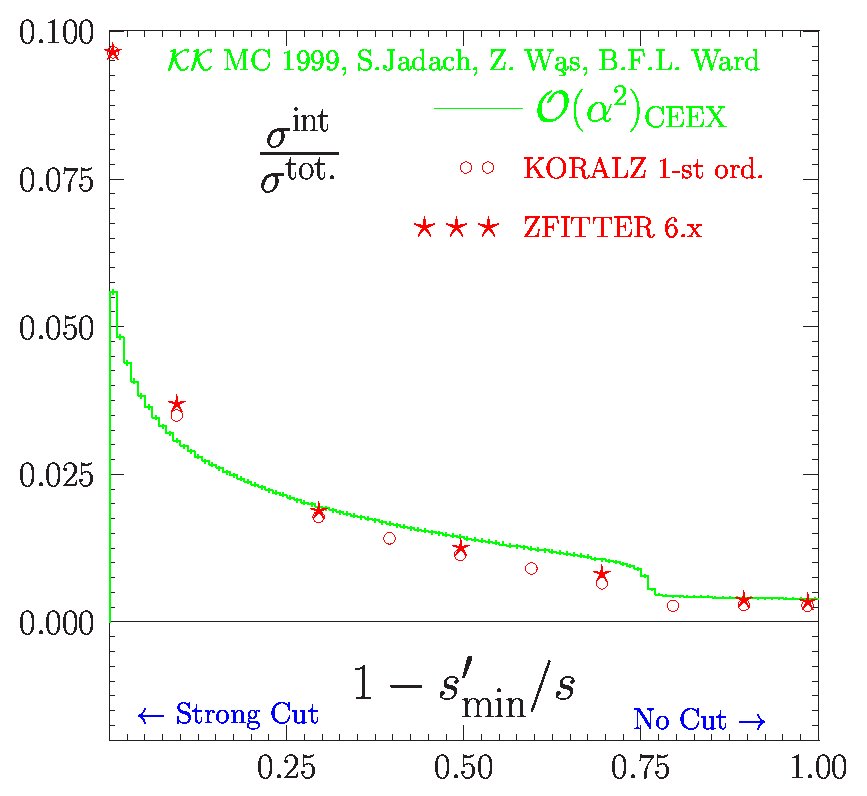
\epsfig{file=afb-int-sig1.eps,width=65mm,height=60mm}
}}
\end{picture}
\end{center}

\end{PSlide}
                                                         %%%%%%%%%%%%%%%%%%%%
%%%%%%%%%%%%%%%%%%%%%%%%%%%%%%%%%%%%%%%%%%%%%%%%%%%%%%%%%%%%%%%%%%%%%%%%%%%%%




%%%%%%%%%%%%%%%%%%%%%%%%%%%%%%%%%%%%%%%%%%%%%%%%%%%%%%%%%%%%%%%%%%%%%%%%%%%%%
%%%%%%%%%%%%%%%%%%%%%%%%%%%%%%%%%%%%%%%%%%%%%%%%%%%%%%%%%%%%%%%%%%%%%%%%%%%%%
%%%%%%%%%%%%%%%%%%%%%%%%%%%%%%%%%%%%%%%%%%%%%%%%%%%%%%%%%%%%%%%%%%%%%%%%%%%%%
                                                         %%%%%%%%%%%%%%%%%%%%
\begin{PSlide}{{\small\color{Magenta} 
      ISR*FSR in $A_{FB}$, energy cut-off study}}

{\small\color{ForestGreen}
  The ISR*FSR {\color{Red} interference} correction
  to $A_{FB}$ at \Energy.
  No cut in $\cos$\Angle.
  From {\color{red} \KK\ M.C. with \Oceex{\alpha^1} }
  exponentiation at the amplitude level.
}

\begin{center}
\setlength{\unitlength}{1mm}
\begin{picture}(65,60)
%#####\put(0,0){\framebox( 65,60){ }}
\put(-2, 00){\makebox(0,0)[lb]{
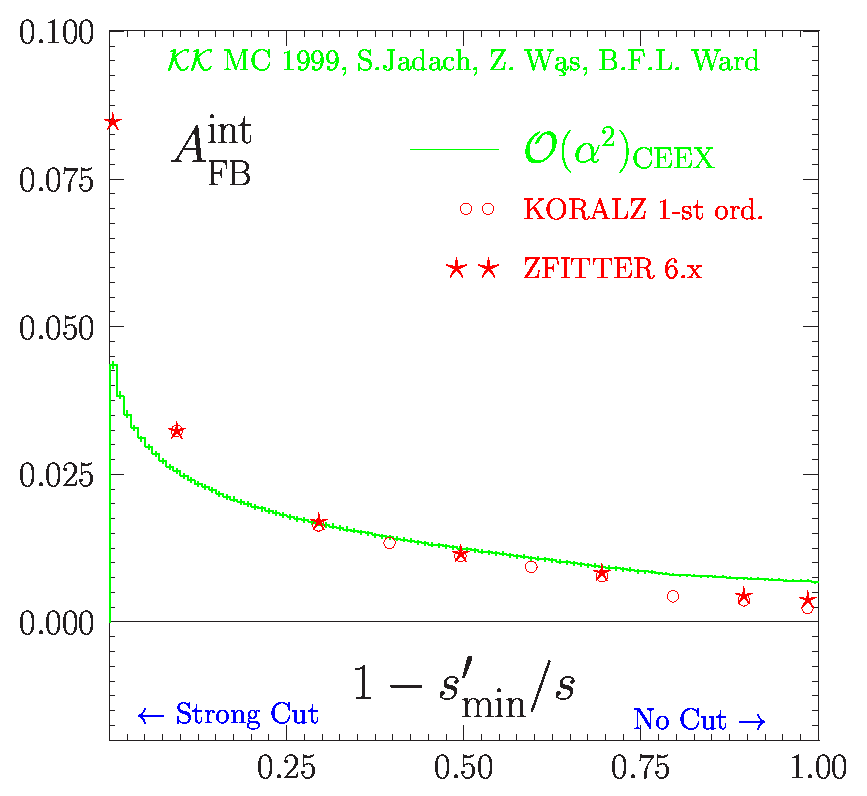
\epsfig{file=afb-int-afb1.eps,width=65mm,height=60mm}
}}
\end{picture}
\end{center}

\end{PSlide}
                                                         %%%%%%%%%%%%%%%%%%%%
%%%%%%%%%%%%%%%%%%%%%%%%%%%%%%%%%%%%%%%%%%%%%%%%%%%%%%%%%%%%%%%%%%%%%%%%%%%%%

%%%%%%%%%%%%%%%%%%%%%%%%%%%%%%%%%%%%%%%%%%%%%%%%%%%%%%%%%%%%%%%%%%%%%%%%%%%%%
%%%%%%%%%%%%%%%%%%%%%%%%%%%%%%%%%%%%%%%%%%%%%%%%%%%%%%%%%%%%%%%%%%%%%%%%%%%%%
%%%%%%%%%%%%%%%%%%%%%%%%%%%%%%%%%%%%%%%%%%%%%%%%%%%%%%%%%%%%%%%%%%%%%%%%%%%%%
                                                         %%%%%%%%%%%%%%%%%%%%
\begin{PSlide}{{\small\color{Magenta} 
      ISR*FSR in $A_{FB}$, energy cut-off study}}

{\small\color{ForestGreen}
  Bin-per-bin  $s'$-dependence of $A_{FB}$ \\
  -- the~ISR*FSR {\color{Red} interference} contribution at \Energy.\\
  Results from {\color{red} \KK\ M.C. with \Oceex{\alpha^1} }
  exponentiation at the amplitude level.\\
  No cut in $\cos$\Angle.
}

\begin{center}
\setlength{\unitlength}{1mm}
\begin{picture}(65,60)
%#####\put(0,0){\framebox( 65,60){ }}
\put(-2, 00){\makebox(0,0)[lb]{
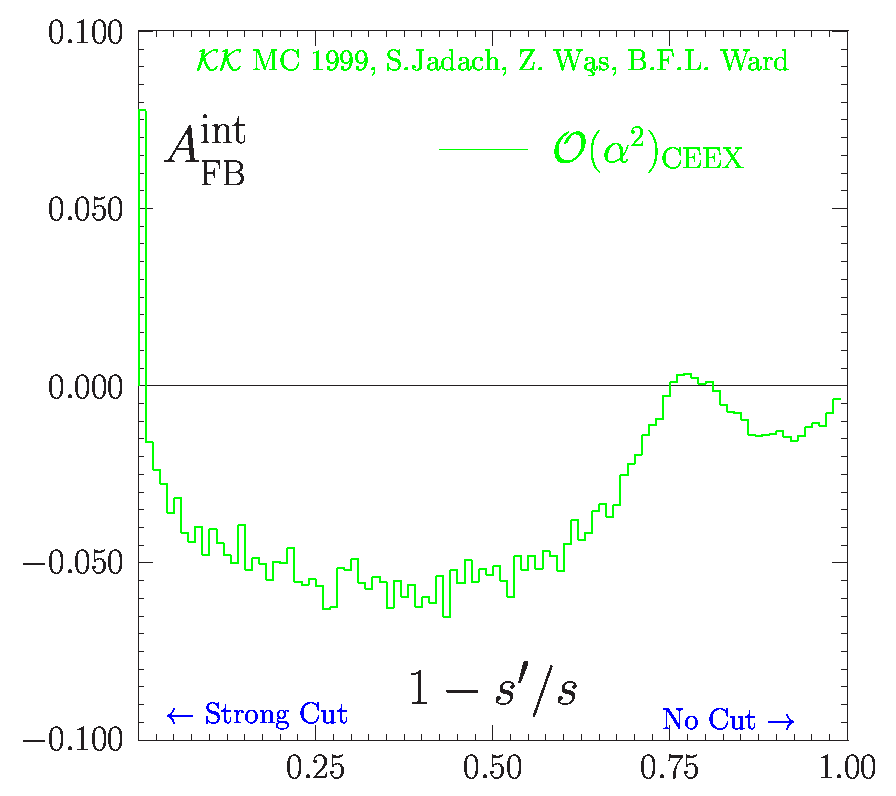
\epsfig{file=afb-int-afb2.eps,width=65mm,height=60mm}
}}
\end{picture}
\end{center}

\end{PSlide}
                                                         %%%%%%%%%%%%%%%%%%%%
%%%%%%%%%%%%%%%%%%%%%%%%%%%%%%%%%%%%%%%%%%%%%%%%%%%%%%%%%%%%%%%%%%%%%%%%%%%%%








%%%%%%%%%%%%%%%%%%%%%%%%%%%%%%%%%%%%%%%%%%%%%%%%%%%%%%%%%%%%%%%%%%%%%%%%%%%%%
%%%%%%%%%%%%%%%%%%%%%%%%%%%%%%%%%%%%%%%%%%%%%%%%%%%%%%%%%%%%%%%%%%%%%%%%%%%%%
%%%%%%%%%%%%%%%%%%%%%%%%%%%%%%%%%%%%%%%%%%%%%%%%%%%%%%%%%%%%%%%%%%%%%%%%%%%%%
                                                         %%%%%%%%%%%%%%%%%%%%
\begin{PSlide}{{\small\color{Magenta} 
      ISR*FSR interf. Realistic acceptance}}

{\small\color{Blue}
  The influence of ISR*FSR  interference at \Energy. 
  The energy cut is on $v_p=1-Q^2_{Aleph}/s$, where $Q^2_{Aleph}$ 
  is s-channel propagator variable of ALEPH.
  The angular cut is $|\cos\theta|<\cos\theta_{\max}$}
{\small\color{Blue} Scattering angle is $\theta=$\Angle. }
{\tiny\color{Blue}  [Angle $\theta^{\bullet}$ is defined in Phys. Rev. {\bf D41}, 1425 (1990)]}

%-----------------------------------------------------------
\begin{center}
\setlength{\unitlength}{1mm}
%
\begin{picture}(35,35)
\put(-1, 0){\makebox(0,0)[lb]{
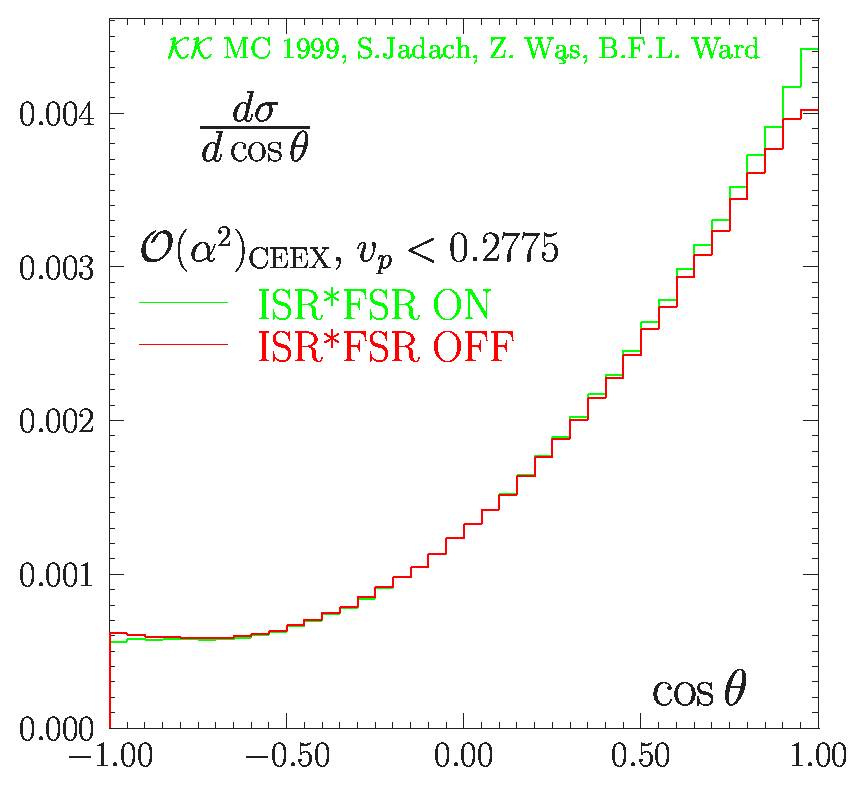
\epsfig{file=afb-int-G1xxx.eps,width=35mm,height=34mm}
}}\end{picture}
%
\begin{picture}(35,35)
\put(-1, 0){\makebox(0,0)[lb]{
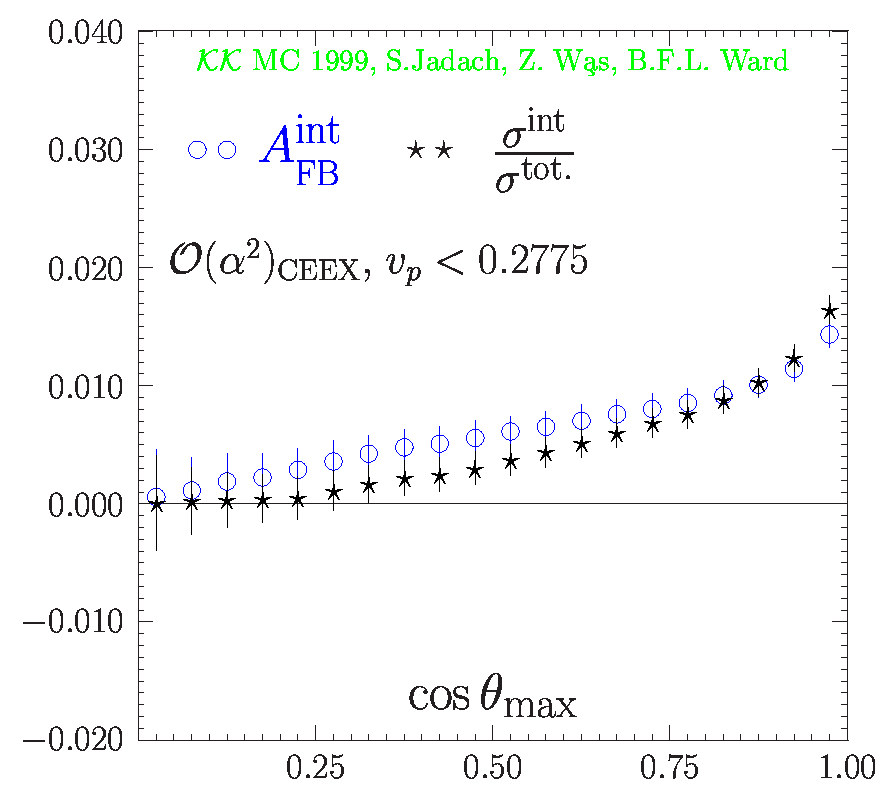
\epsfig{file=afb-int-com1xxx.eps,width=35mm,height=34mm}
}}\end{picture}
%
\end{center}
%-----------------------------------------------------------
\end{PSlide}
                                                         %%%%%%%%%%%%%%%%%%%%
%%%%%%%%%%%%%%%%%%%%%%%%%%%%%%%%%%%%%%%%%%%%%%%%%%%%%%%%%%%%%%%%%%%%%%%%%%%%%





%%%%%%%%%%%%%%%%%%%%%%%%%%%%%%%%%%%%%%%%%%%%%%%%%%%%%%%%%%%%%%%%%%%%%%%%%%%%%
%%%%%%%%%%%%%%%%%%%%%%%%%%%%%%%%%%%%%%%%%%%%%%%%%%%%%%%%%%%%%%%%%%%%%%%%%%%%%
%%%%%%%%%%%%%%%%%%%%%%%%%%%%%%%%%%%%%%%%%%%%%%%%%%%%%%%%%%%%%%%%%%%%%%%%%%%%%
                                                         %%%%%%%%%%%%%%%%%%%%
\begin{PSlide}{{\small\color{Magenta} 
      ISR*FSR interf. Realistic acceptance}}

{\small\color{Blue}
  The influence of ISR*FSR interference at \Energy. 
  The energy cut is on $v_p=1-Q^2_{Aleph}/s$, where $Q^2_{Aleph}$ 
  is s-channel propagator variable of ALEPH.
  No angular cut.}
%-----------------------------------------------------------
\begin{center}
\setlength{\unitlength}{1mm}
%
\begin{picture}(35,35)
\put(-1, 0){\makebox(0,0)[lb]{
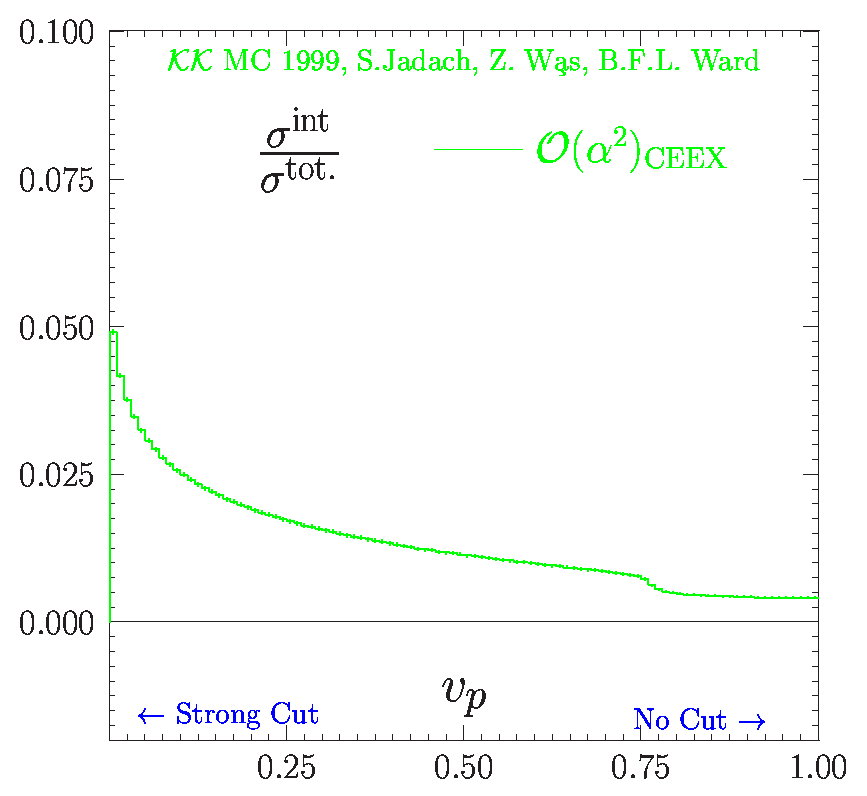
\epsfig{file=afb-int-sig1S.eps,width=35mm,height=34mm}
}}\end{picture}
%
\begin{picture}(35,35)
\put(-1, 0){\makebox(0,0)[lb]{
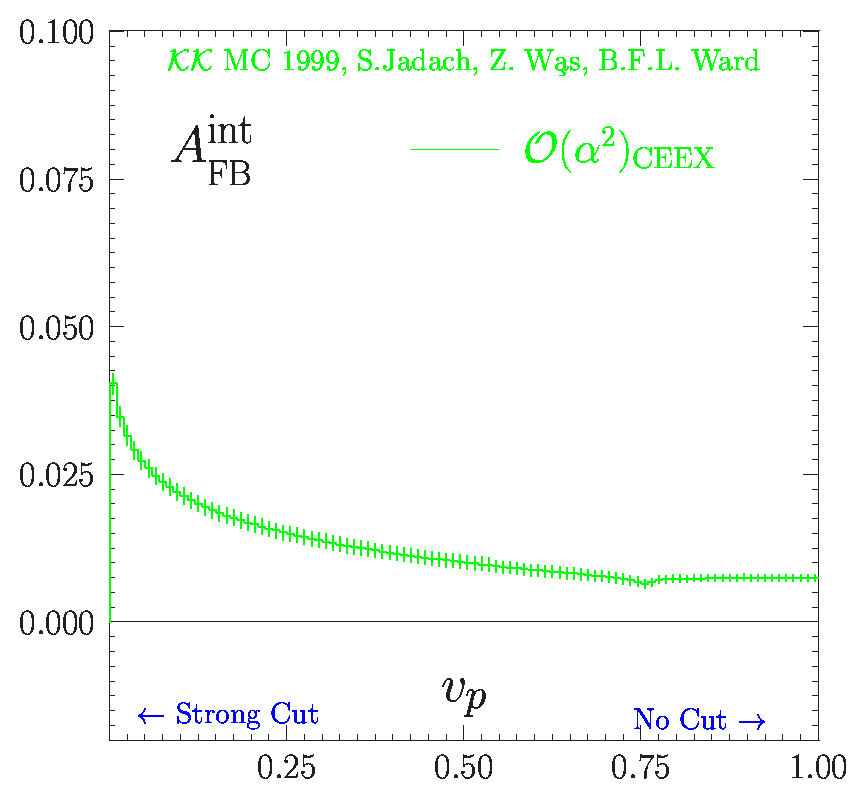
\epsfig{file=afb-int-afb1S.eps,width=35mm,height=34mm}
}}\end{picture}
%
\end{center}
%-----------------------------------------------------------
\end{PSlide}
                                                         %%%%%%%%%%%%%%%%%%%%
%%%%%%%%%%%%%%%%%%%%%%%%%%%%%%%%%%%%%%%%%%%%%%%%%%%%%%%%%%%%%%%%%%%%%%%%%%%%%






%%%%%%%%%%%%%%%%%%%%%%%%%%%%%%%%%%%%%%%%%%%%%%%%%%%%%%%%%%%%%%%%%%%%%%%%%%%%%
%%%%%%%%%%%%%%%%%%%%%%%%%%%%%%%%%%%%%%%%%%%%%%%%%%%%%%%%%%%%%%%%%%%%%%%%%%%%%
%%%%%%%%%%%%%%%%%%%%%%%%%%%%%%%%%%%%%%%%%%%%%%%%%%%%%%%%%%%%%%%%%%%%%%%%%%%%%
                                                         %%%%%%%%%%%%%%%%%%%%
\begin{PSlide}{{\small\color{Magenta} 
      ISR*FSR interf. KORALZ 1-st order}}

{\small\color{Blue}
  The influence of ISR*FSR  interference at \Energy. 
  The energy cut is on $s'/s$, where $s'=m^2_{f\bar{f}}$.
  The angular cut is $|\cos\theta|<\cos\theta_{\max}$}
{\small\color{Blue} Scattering angle is $\theta=$\Angle. }
{\tiny\color{Blue}  [Angle $\theta^{\bullet}$ is defined in Phys. Rev. {\bf D41}, 1425 (1990)]}

%-----------------------------------------------------------
\begin{center}
\setlength{\unitlength}{1mm}
%
\begin{picture}(35,35)
\put(-1, 0){\makebox(0,0)[lb]{
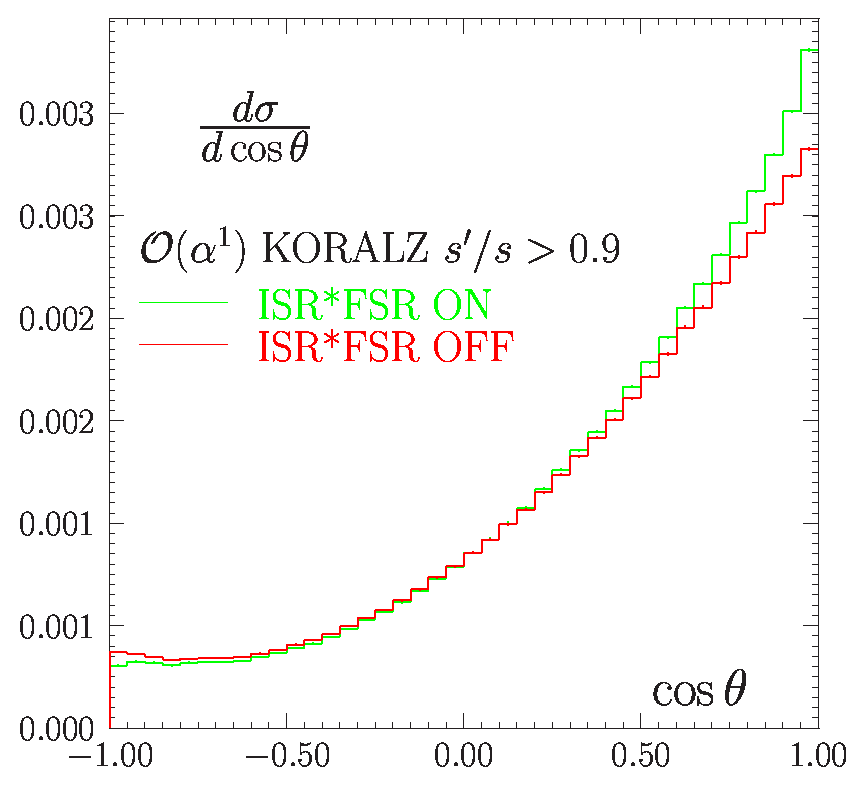
\epsfig{file=afb-int-AngMx.eps,width=35mm,height=34mm}
}}\end{picture}
%
\begin{picture}(35,35)
\put(-1, 0){\makebox(0,0)[lb]{
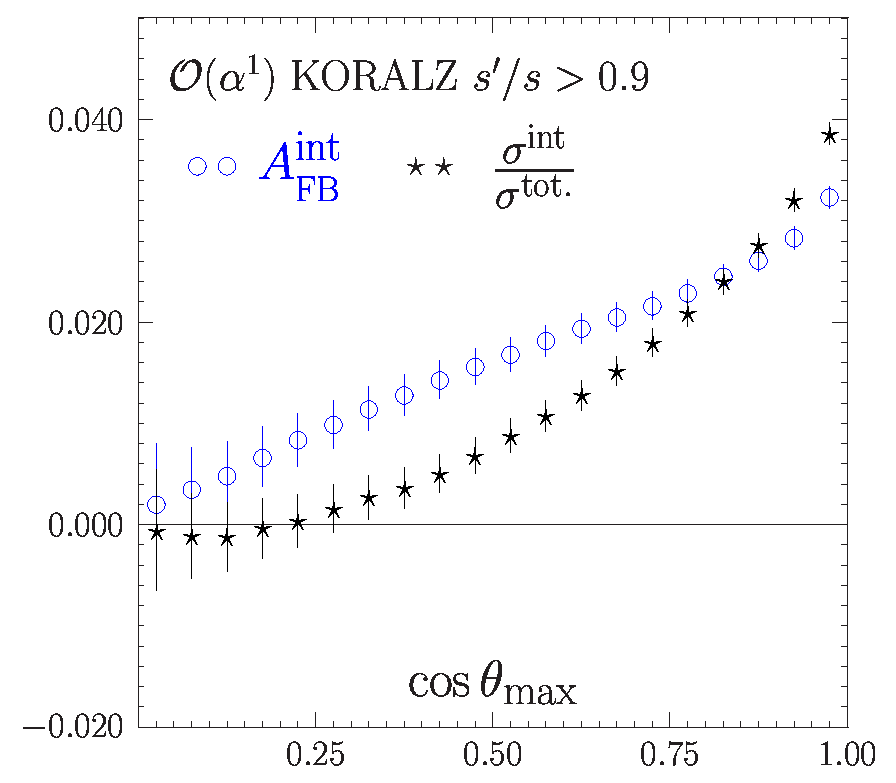
\epsfig{file=afb-int-comMx.eps,width=35mm,height=34mm}
}}\end{picture}
%
\end{center}
%-----------------------------------------------------------
\end{PSlide}
                                                         %%%%%%%%%%%%%%%%%%%%
%%%%%%%%%%%%%%%%%%%%%%%%%%%%%%%%%%%%%%%%%%%%%%%%%%%%%%%%%%%%%%%%%%%%%%%%%%%%%










%%%%%%%%%%%%%%%%%%%%%%%%%%%%%%%%%%%%%%%%%%%%%%%%%%%%%%%%%%%%%%%%%%%%%%%%%%%%%
%%%%%%%%%%%%%%%%%%%%%%%%%%%%%%%%%%%%%%%%%%%%%%%%%%%%%%%%%%%%%%%%%%%%%%%%%%%%%
%%%%%%%%%%%%%%%%%%%%%%%%%%%%%%%%%%%%%%%%%%%%%%%%%%%%%%%%%%%%%%%%%%%%%%%%%%%%%
                                                         %%%%%%%%%%%%%%%%%%%%
\begin{Slide}{{\bf\color{red} Appendix: \KK\ versus our older MC's and plans}}

   %%%%%%%%%%%%%%%%%%%%%%%%%%%%%%%%%%%%%%%%%%%%%%%%%%%%%%%%%%%%
   %%%         LIST OF FEATURES OF KK MC                    %%%
   %%%%%%%%%%%%%%%%%%%%%%%%%%%%%%%%%%%%%%%%%%%%%%%%%%%%%%%%%%%%

\vspace{-2mm}
{\scriptsize
\begin{center}
\begin{tabular}{|p{17mm}|l|l|l|l|}
\hline\hline
Feature & KORALB &KORALZ & ${\cal KK}$ now & ${\cal KK}$ 2000\\ 
\hline\hline%----------------------------------------------------------------
%
ISR  & $\alpha+\alpha L$ & {\tiny $(\alpha+\alpha L+\alpha^2 L^2)_{_{\rm exp}}$} 
                         & {\tiny\color{red} $(...+\alpha^3 L^3)_{_{\rm exp}}$}             
                         & {\tiny $(...+\alpha^3 L^3)_{_{\rm exp}}$} \\
\hline%----------------------------------------------------------------------
FSR  & $\alpha+\alpha L$ & {\tiny $(\alpha+\alpha L+\alpha^2 L^2)_{_{\rm exp}}$} 
                         & {\tiny $(...+\alpha^2 L^2)_{_{\rm exp}}$}             
                         & {\tiny $(...+\alpha^3 L^3)_{_{\rm exp}}$} \\
\hline%----------------------------------------------------------------------
{\tiny ISR*FSR interf.}  & {\tiny $\alpha+\alpha L$} 
                      & {\tiny $\alpha+\alpha L$, no exp.} 
                      & {\tiny\color{red} $(\alpha+\alpha L)_{_{\rm exp}}$}
                      & {\tiny            $(\alpha+\alpha L)_{_{\rm exp}}$}\\
\hline%----------------------------------------------------------------------
{\tiny Exponentiation}   &  NONE  & for $|M(p_i)|^2$   
                                  & {\color{red}for $M(p_i)$}   
                                  & {\color{red}for $M(p_i)$}   \\
\hline%----------------------------------------------------------------------
{\tiny Exact m.el. for real photons} 
                       & up to 1  & 1, 2coll.   & 1, 2coll, 3coll.   & {\color{red}up to 3 } \\
\hline%----------------------------------------------------------------------
El-Weak              & No Z-reson.   & YES   & YES   & YES  \\
\hline%----------------------------------------------------------------------
\hline%----------------------------------------------------------------------
{\tiny Beam polar.}  & {\tiny long+trans.}   
                     & longit.   & {\color{red} long+trans.}   & {\color{red} long+trans.}   \\
\hline%----------------------------------------------------------------------
$\tau$ polar.        & {\tiny long+trans.}   
                     & longit.   & {\color{red} long+trans.}   &  {\color{red} long+trans.}  \\
\hline%----------------------------------------------------------------------
\hline%----------------------------------------------------------------------
{\tiny Hadronization}   & ---   & Yes   & Yes               &  Yes   \\
\hline%----------------------------------------------------------------------
$\tau$ decay            & Yes   & Yes   &  Yes              &  Yes   \\
\hline%----------------------------------------------------------------------
{\tiny Inclusive mode}  & ---   & No    & Yes               &  Yes   \\
\hline%----------------------------------------------------------------------
{\tiny Beamstrahlung}   & ---   & No    & {\color{red} Yes} &  Yes   \\
\hline%----------------------------------------------------------------------
{\tiny beam spread}     & ---   & No    & Yes               &  Yes   \\
\hline%----------------------------------------------------------------------
\hline%----------------------------------------------------------------------
{\tiny $\nu\nu$ channel}& ---   & Yes   & {\color{red} No}  &  Yes   \\
\hline%----------------------------------------------------------------------
{\tiny $ee$ channel}    & ---   & No    & {\color{red} No}  &  Yes   \\
\hline%----------------------------------------------------------------------
{\tiny $tt$ channel}    & ---   & No    & No                &  ???   \\
\hline%----------------------------------------------------------------------
{\tiny $WW$ channel}    & ---   & No    & No                &  ???   \\
\hline\hline%----------------------------------------------------------------
\end{tabular}
\end{center}
}

\end{Slide}                               %%%%%%%%%%%%%%%%%%%%%%%%%%%%%%%%%%
%%%%%%%%%%%%%%%%%%%%%%%%%%%%%%%%%%%%%%%%%%%%%%%%%%%%%%%%%%%%%%%%%%%%%%%%%%%%%









%%%%%%%%%%%%%%%%%%%%%%%%%%%%%%%%%%%%%%%%%%%%%%%%%%%%%%%%%%%%%%%%%%%%%%%%%%%%%
%%%%%%%%%%%%%%%%%%%%%%%%%%%%%%%%%%%%%%%%%%%%%%%%%%%%%%%%%%%%%%%%%%%%%%%%%%%%%
                                                         %%%%%%%%%%%%%%%%%%%%
\begin{Slide}{{\bf\color{red} Conclusions }}

\vspace{-2mm}
{\bf\color{blue}
  \KK\ Monte Carlo and KORALZ answers on ISR*FSR Interference:\\
  \begin{itemize}
  \item
    For typical exp. energy cut 0.3 ISR*FSR int. is about 1.5\% in $\sigma_{tot}$ and $A_{FB}$.
  \item
    For energy cut 0.1 it is twice bigger.
  \item
    The cut $|\cos\theta<0.9$ makes it 25\% smaller.
  \item
    The \Order{\alpha^1} ISR*FSR int. is under total controll using KORALZ and \KK\ Monte Carlo
    for arbitrary cuts.
  \item
    Effects beyond \Order{\alpha^1} are negligible, ($<$20\% of \Order{\alpha^1}),
    except when energy cut is stronger than 0.1.
  \item
    ISR*FSR int. at Z radiative return is very small, as expected.
  \item
    Change from $s'$ to $Q^2$-propagator in energy cut has no effect.
  \end{itemize}
}


\end{Slide}                               %%%%%%%%%%%%%%%%%%%%%%%%%%%%%%%%%%%
%%%%%%%%%%%%%%%%%%%%%%%%%%%%%%%%%%%%%%%%%%%%%%%%%%%%%%%%%%%%%%%%%%%%%%%%%%%%%







\end{document}                                           %%%%%%%%%%%%%%%%%%%%
%%%%%%%%%%%%%%%%%%%%%%%%%%%%%%%%%%%%%%%%%%%%%%%%%%%%%%%%%%%%%%%%%%%%%%%%%%%%%
%%%%%%%%%%%%%%%%%%%%%%%%%%%%%%%%%%%%%%%%%%%%%%%%%%%%%%%%%%%%%%%%%%%%%%%%%%%%%


(cp afb-int-G1.eps    Lep2wgTalk/  ;
 cp afb-int-com1.eps  Lep2wgTalk/  ;
 cp afb-int-G1x.eps   Lep2wgTalk/  ;
 cp afb-int-com1x.eps Lep2wgTalk/  ;
 cp afb-int-sig1.eps  Lep2wgTalk/  ;
 cp afb-int-afb1.eps  Lep2wgTalk/  ;
 cp afb-int-afb2.eps  Lep2wgTalk/  ;
 cp afb-int-G1xxx.eps Lep2wgTalk/  ;
 cp afb-int-com1xxx.eps Lep2wgTalk/  ;
 cp afb-int-sig1S.eps Lep2wgTalk/  ;
 cp afb-int-afb1S.eps Lep2wgTalk/  ;
 cp afb-int-AngMx.eps Lep2wgTalk/  ;
 cp afb-int-comMx.eps Lep2wgTalk/  )
gtar -cvzf Lep2wgTalk.tar.gz Lep2wgTalk
